\section{Design}


We aim to evade advanced phishing websites from the user end in real time when users visit them by triggering the fingerprinting cloaking techniques.
To this end, we design, implement, and evaluate~\spartacus, a framework that automatically cloaks users and hence evades malicious websites that implement fingerprint cloaking.

\begin{figure*}
\centering
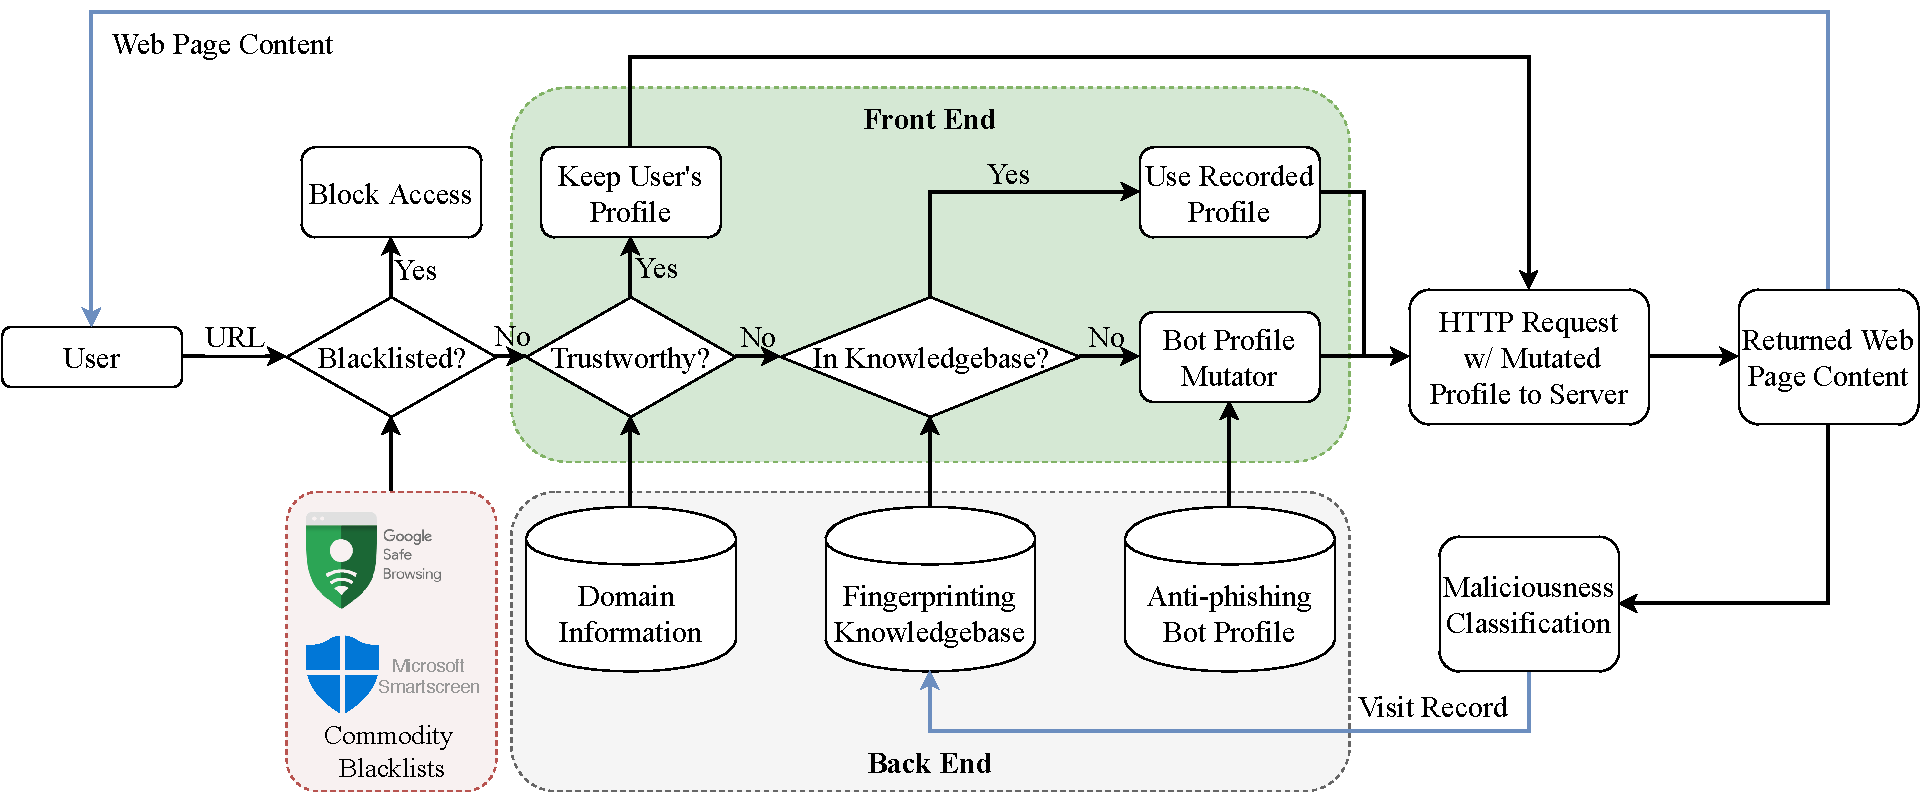
\includegraphics[width=\linewidth]{figs/arch.pdf}
\caption{\spartacus architecture.}
\label{fig:sp_arch}
% \vspace{-10pt}
\end{figure*}

\subsection{Overview}
\autoref{fig:sp_arch} demonstrates the architecture of the \spartacus system.
The whole system consists of two parts, \emph{front end} and \emph{back end}. 
The front end is responsible for filtering already blacklisted URLs and mutating profiles in the HTTP request such as user agent.
\spartacus also checks the information of benign websites to decide whether to mutate the profile.
In the back end, we maintain several databases to provide support to the front end, including black and whitelist database, which is used to process known URLs, fingerprinting knowledge base, which stores the successful mutation, the anti-phishing bot profile database, which contains the profiles of anti-phishing systems such as google bot, phishing attributes, which is used to distinguish the maliciousness of returned web page content. 

When a user tries to visit a URL, first the URL goes to black and whitelist. 
If the existing record is found, the browser will either block the access or keep user's original profile when requesting the server. 
Otherwise, the front end will query the fingerprinting knowledgebase to see if we have processed the same url before, if found, we will use recorded profile to request the website, if not, we will mutate profile to a bot one. Then with the “spartacus” profile, HTTP request is sent to the server. After getting the page content, we determine whether there is maliciousness. If yes, the browser will show a warning sign to the user, or the web page content will be shown to the user. The knowledge base will be updated accordingly under both situations. 

\subsection{Collection and Maintenance of Back End Databases}

\noindent
\textbf{Blacklist database.}
Blacklist based anti-phishing systems such as Google Safe Browsing and Microsoft SmartScreen have been examining and collecting phishing URLs to warn users before they visit the websites.
We collect known phishing URLs from common blacklists so that \spartacus can leverage the achievements from the anti-phishing systems to facilitate the web request process when dealing with known phishing websites.
% Similarly, we leverage a whitelist to avoid any impacts brought by \spartacus so that the users can visit legitimate websites with their own profiles.

\noindent
\textbf{Fingerprinting Knowledgebase.}
The fingerprinting knowledgebase is shared among users who leverage \spartacus and stores profiles with which users cannot see malicious content when requesting the server.
After the maliciousness classification, if phishing content is not found in the responded source, then we mark the mutated profile used in the request this time, connect it with the URL, and update the pair as success into the knowledgebase.
When other users try to visit the same URL, \spartacus will use the corresponding profile recorded in the database to guarantee that users do not receive malicious content.

\noindent
\textbf{Anti-phishing Bot Profile Database.}
The profiles of anti-phishing system crawlers are keeping updating all the time.
Accordingly, phishers refresh their blacklist to precisely evade the access from the anti-phishing bots.
Therefore, we crawl the up-to-date profiles of anti-phishing systems into the database and hence \spartacus can leverage them to visit suspicious websites and receive benign web page content.

% \noindent
% \textbf{Phishing Attribute Database.}
% After sending request with mutated profile and receiving respond from the server, \spartacus needs to classify whether maliciousness exists in the web page content.
% It implements the state-of-the-art phishing detections such as content-based and visual-similarity-based methodologies to extract phishing attributes based on the responded web page content such as screenshots and HTML source code.
% \spartacus compares such features with those from websites of most phishing-targeted organizations, which stores in the Phishing Attribute Datatbase.


\subsection{Benign Domain Handling}

We preliminarily tested how \spartacus works on benign websites to figure out the optimal methodology that can bring negligible impact on them.
Among 60,848 benign websites that \spartacus visited, 150 of them blocked the access from a browser with \spartacus.
To make benign websites allow the visit with \spartacus while keeping its evasion ability against advanced phishing websites,
% To further differentiate between a legitimate anti-bot page and a phishing one that appears due to cloaking,
we extract domain reputation~\cite{reputation}, registration duration~\cite{whois}, and top viewed sub-domains~\cite{topviewedsubdomains} of URLs from false-positive (FP) and true-positive (TP) sides.
Cisco defines reputation of a domain as five categories: Trusted, Favorable, Neutral, Questionable, and Untrusted.
We inspect 150 URLs on each side.
Reputation-wise, 136 out of 150 TP URLs --- phishing --- have reputation lower or equal to Neutral level, the lowest of which is Poor Verdict.
In contrast, 24 of 150 FP URLs reside lower than Favorable level, the lowest of which is Questionable (only one).
In terms of domain lifespan, the mean value of domain duration since registration for FP URLs is 4,692 days and the median is 4,521 days.
However, the average lifespan of the malicious domains is 1,618 days, with median of 900 days.
Moreover, all 150 FP URLs fall into the top viewed sub-domains of the corresponding domain names, but none of the TP ones matches with them.

From the evaluation result, we summarize that a legitimate domain has a higher reputation and longer life than a malicious one, and they are within top viewed sub-domains.
With the finding, we can further reduce the FPs of \spartacus by querying the attributes of the domain to decide whether to mutate the HTTP profile.
We choose the phishing domain duration that resides on 75\% in the list (1,501) and Neutral level as threshold.
If one URL has a lifespan lower than 1,501 days and its reputation level is Neutral or worse, or its sub-domain is not top viewed, \spartacus will mutate the HTTP profile before request.
The logic is shown in~\Cref{alg:mutatelogic}.

\begin{algorithm}\captionsetup{labelfont={sc,bf}, labelsep=newline}
  \caption{Logic of mutating HTTP profile}
\begin{algorithmic}[1]

\State $p_d = default\_profile$
\State $u = url\_to\_visit$

\If{\State $reputation(u)~\leq Neutral$ \texttt{and}
\State $duration(u)~\geq 1,501$ \texttt{or} 
\State $d.domain$ NOT in top reviewed sub-domains}
    \State $p_n = mutate\_http\_profile(p_d)$
\EndIf

\State $send\_request(p_n)$

\end{algorithmic}
\label{alg:mutatelogic}
\end{algorithm}


\subsection{Decision Makers on A URL Visit}

When a user attempts to visit a URL, the URL will go through several decision makers to assure a safe browsing.
The decision makers consist of Blacklist Filter, Whitelist Filter, Knowledgebase Query, and Maliciousness Classification.
We will elaborate them in order of the system flow.

\noindent
\textbf{Blacklist Filter.}
With the contribution of the anti-phishing ecosystem, \spartacus can filter known phishing URLs through the query to the Malicious URL BlackList Database.
Any match in the blacklist database will result in a block access to the URL without further action.

% \noindent
% \textbf{Whitelist Filter.}
% Similar to the blacklist filter, the whitelist filter in \spartacus helps filter the whitelisted URLs so that the user can receive the web page content with best out-looking that the organization configures to fit in the visit from different browsers or devices.

\noindent
\textbf{Knowledgebase Query.}
When the URL does not fall into either Blacklist or Whitelist filter, \spartacus will examine whether such URL has been visited once by either the user or other users by querying the Fingerprinting Knowledgebase.
If a record is found in the knowledgebase, \spartacus will mutate the web request profile according to the record to make sure that such web request profile will return a benign web page content;
otherwise, \spartacus will call a \emph{Bot Profile Mutator}, which randomly selects one profile from Anti-phishing Bot Profile Database to submit the web request and lowers the impact to possible web page layout to the lowest.



\subsection{Bot Profile Mutator}

It is the Bot Profile Mutator that takes responsibility of profile mutation to evade malicious content in advanced phishing websites.
There are several items in the HTTP profile that can be modified or changed to camouflage the user as anti-phishing crawlers.
Take User-Agent as an example. 
Generally, anti-phishing crawlers contain ``bot'', ``crawler'', or the name of the company such as ``Google'', ``PayPal'' in the User-Agent string.
We name the words that can trigger the cloaking technique in phishing attacks as \emph{triggering words}.
Scripts in the phishing server typically read the string from HTTP requests and filter visits that contain crawler-like patterns.
Another instance is Referer, where the visit is from previously.
Typically the previous location for a potential victim is from phishing lures the attackers distributed earlier.
Hence, phishers can block all visits who are not from the phishing lures.

To take advantage of phisher's filtering algorithm, the Bot Profile Mutator modifies the identifiable items in the HTTP profile such as User-Agent and Referer before the browser sends out the request.
In detail, after querying from the Fingerprinting Knowledgebase, \spartacus will append the successful sensitive word in the knowledgebase to user's own User-Agent string.
It also checks the necessity of mutation of Referer within the same record.
If there is no successful record in the database,
the mutator will randomly choose one word from a list of 407 triggering words.
Additionally, it set the Referer to either None or ``www.google.com'' to further pretend the user as anti-phishing crawler.
% 407 sensitive words


% \subsubsection{Maliciousness Classification.}
\noindent
\textbf{Maliciousness Classification.}
After submitting the web request to the server, \spartacus along with the browser will receive a response from the server.
There are different situations of the response as follows:

\begin{itemize}
    \item The server responds either a benign page or an error page with status code of 4XX/5XX, or, it redirects the visit to a benign website, which is typically the website it impersonates;
    \item The server returns malicious web page content.
\end{itemize}


The former result is because (a) the server is malicious with evasion techniques and determines the visit from \spartacus as anti-phishing bot visit, or (b) the website is benign itself.
The latter one is caused by (a) a malicious website without evasion techniques, or (b) a malicious website with evasion techniques, which is not triggered by the mutated profile from \spartacus.

The latter situation is what \spartacus needs to handle.
As for reason (a), \spartacus relies on the current anti-phishing systems that are well capable of detecting basic phishing websites within a short time period and hence the whole ecosystem can be protected from such phishing attacks.
For reason (b), the phishing website implements evasion techniques that remain unknown after one visit.
However, as \spartacus can be used by a large number of users, there is high possibility where a number of users will visit the same URL.
\spartacus learns from different attempts of mutations of web request profiles that failed to trigger cloaking in the Fingerprinting Knowledgebase.
Avoiding using the failed ones, \spartacus mutates the profile with new triggering words from the list, and hence we can eventually fingerprint the trigger of the evasion technique in the phishing website and apply such configuration for all \spartacus users who visit the same URL.
Before \spartacus figures out the cloaking technique, it implements visual-similarity and content-based phishing detection mechanisms and alerts the user if any of the attributes detected in the content by matching the features with those in Phishing Attribute Database.
% otherwise, the browser user will see a benign web page content.






\section{Privacy}

Note that installing and using \spartacus may lead to the compromise of privacy.
For example, some discount discovery extension may leak the annual income level of users~\cite{honey}.
And some of the VPN services require user's location information and Personal Identifiable Information (PII)~\cite{ZenMate}.
Such privacy information may be leaked and hence abused by attackers.  
We thereby enumerate the privacy information \spartacus collects to support the phishing evading services.

\subsubsection{Privacy Information}

\spartacus require four types of privacy information from users to prevent them from being trapped in advanced phishing websites.
We do not collect any PII in \spartacus and hence can protect user's privacy to maximum extent.

% \noindent
(1)~\emph{URL a user tries to visit}: \spartacus needs it to query the reputation, age of domain, and top reviewed subdomains to determine whether to mutate.
If \spartacus makes the decision to mutate the profile, it also needs the URL to query the Fingerprinting Knowledgebase for successful mutation that can evade malicious content.

% \noindent
(2)~\emph{HTTP profile used in the request}:
After \spartacus decides to mutate the user's HTTP profile before visiting a suspicious website, it requires the user's profile to modify it.
The privacy information in the profile includes the User-Agent string, where browser version, browser type, and operating system information reside, and the Referer, which implies the previous location of the user.
By accessing the profile, \spartacus can modify the fingerprints that phishers identify as anti-phishing crawlers to camouflage users.

% \noindent
(3)~\emph{Returned HTTP response}:
\spartacus requires the returned HTTP response to inspect whether the website still contains maliciousness.
For example, if the response status code is 4XX/5XX, it means that there will not be malicious content.
If there is a 200 content returned,
an external classification process will determine its maliciousness by searching for phishing content such as sensitive words and log in form~\cite{xiang2011cantina+}.
The inspection result marks the corresponding profile mutation successful or not.

(4)~\emph{URL and profile share}:
\spartacus at last uploads the URL and the inspection result along with the corresponding HTTP profile to the server.
When other users visit the same URL, the successful mutation will be shared to them.
If there is no successful variant, \spartacus will avoid to use the unsuccessful ones to mutate.


\subsubsection{Privacy Consent and Protection}

We ensure that our \spartacus system well considers users' privacy information,
so we have both consent and protection methodology to notice users and prevent their information from being stolen and abused.

\noindent
\textbf{Consent.}
To have users be aware of the types of privacy information \spartacus checks and modifies before using it,
we set up a privacy policy consent notice when people first time use \spartacus.
At the beginning of the consent, we summarize the privacy information \spartacus use for user's convenience.
Then, by using Privacy Policies~\cite{privacypolicy}, we create one privacy policy for \spartacus.
We elaborate the information \spartacus collects, how it will be used, and how it will be transferred and shared.
Users can choose to opt out and uninstall our system if they do not agree with the consent.

\noindent
\textbf{Protection Methodology.}
First of all, the privacy information \spartacus collects does not contain any PII, which fundamentally protects users' privacy.
Secondly, when the URL and its corresponding HTTP profile is transferred to the server,
it is hashed first and uploaded to the server.
Lastly, when other users look up existing records from the server,
their URL is also hashed first and looked up in the database in hash version.
Furthermore, what they receive from the Fingerprinting Knowledgebase is whether specific sensitive words can evade maliciousness.
They will not know who exactly ever visited the website.
And hence, the privacy of the user can be protected.